\documentclass[12pt]{article}
\usepackage{graphicx}
\usepackage{amsmath}
\usepackage{hyperref}
\usepackage{listings}
\usepackage{xcolor}
\usepackage{float}

\title{Emotion Detection from Text using the SEMMA Methodology}
\date{\today}

\begin{document}

\maketitle

\begin{abstract}
Emotion detection from text is a pivotal task in natural language processing, essential for understanding human sentiment in various contexts. In this study, we employ the SEMMA methodology to detect emotions from a dataset of tweets. Our findings offer insights into the intricacies of human sentiment and underscore the power of systematic data analysis.
\end{abstract}

\section{Introduction}
Understanding human emotions from textual data plays a critical role in a plethora of applications, ranging from sentiment analysis in customer reviews to modulating chatbot behaviors. The SEMMA methodology, encompassing Sampling, Exploration, Modification, Modeling, and Assessment, provides a structured approach to tackle this complex task. This paper details our journey through these stages using a dataset sourced from Kaggle.

\section{Dataset Description}
The dataset consists of tweets paired with their corresponding emotion labels. Each entry in the dataset provides a short textual snippet, typically representing a sentiment or emotion.

\begin{figure}[h]
\centering
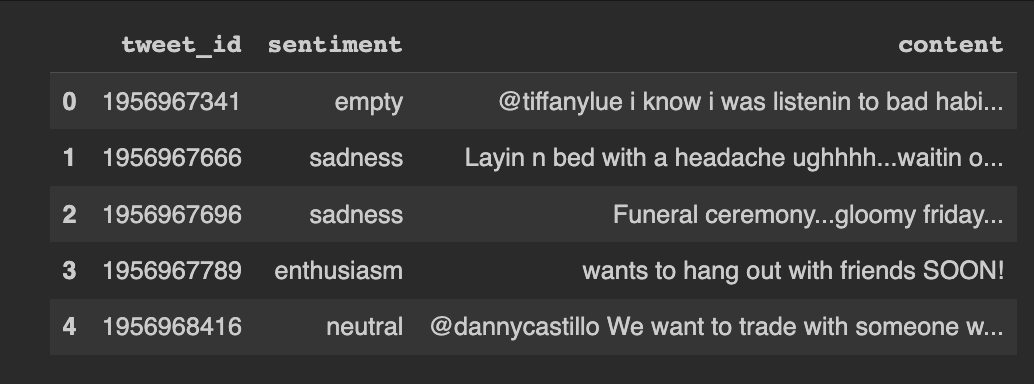
\includegraphics[width=0.8\textwidth]{path_to_sample_data.png}
\caption{Sample data from the dataset}
\end{figure}

\section{Methodology: SEMMA}

\subsection{Sampling}
To achieve computational efficiency without compromising the representation of the dataset, we sampled 80\% of the original dataset. This ensures a balance between computational time and data representation.

\subsection{Exploration}
Exploration is instrumental for understanding the dataset's characteristics and intricacies. Our dataset was devoid of missing values, a rarity in real-world datasets. Additionally, a sentiment distribution analysis was conducted, revealing the presence of potential class imbalances.\\

\textbf{Sentiment Distribution:}\\
Understanding the distribution of the target variable is crucial. A skewed distribution can introduce biases in model predictions. The sentiment distribution in our dataset was visualized to uncover any class imbalances.

\begin{figure}[H]

\centering
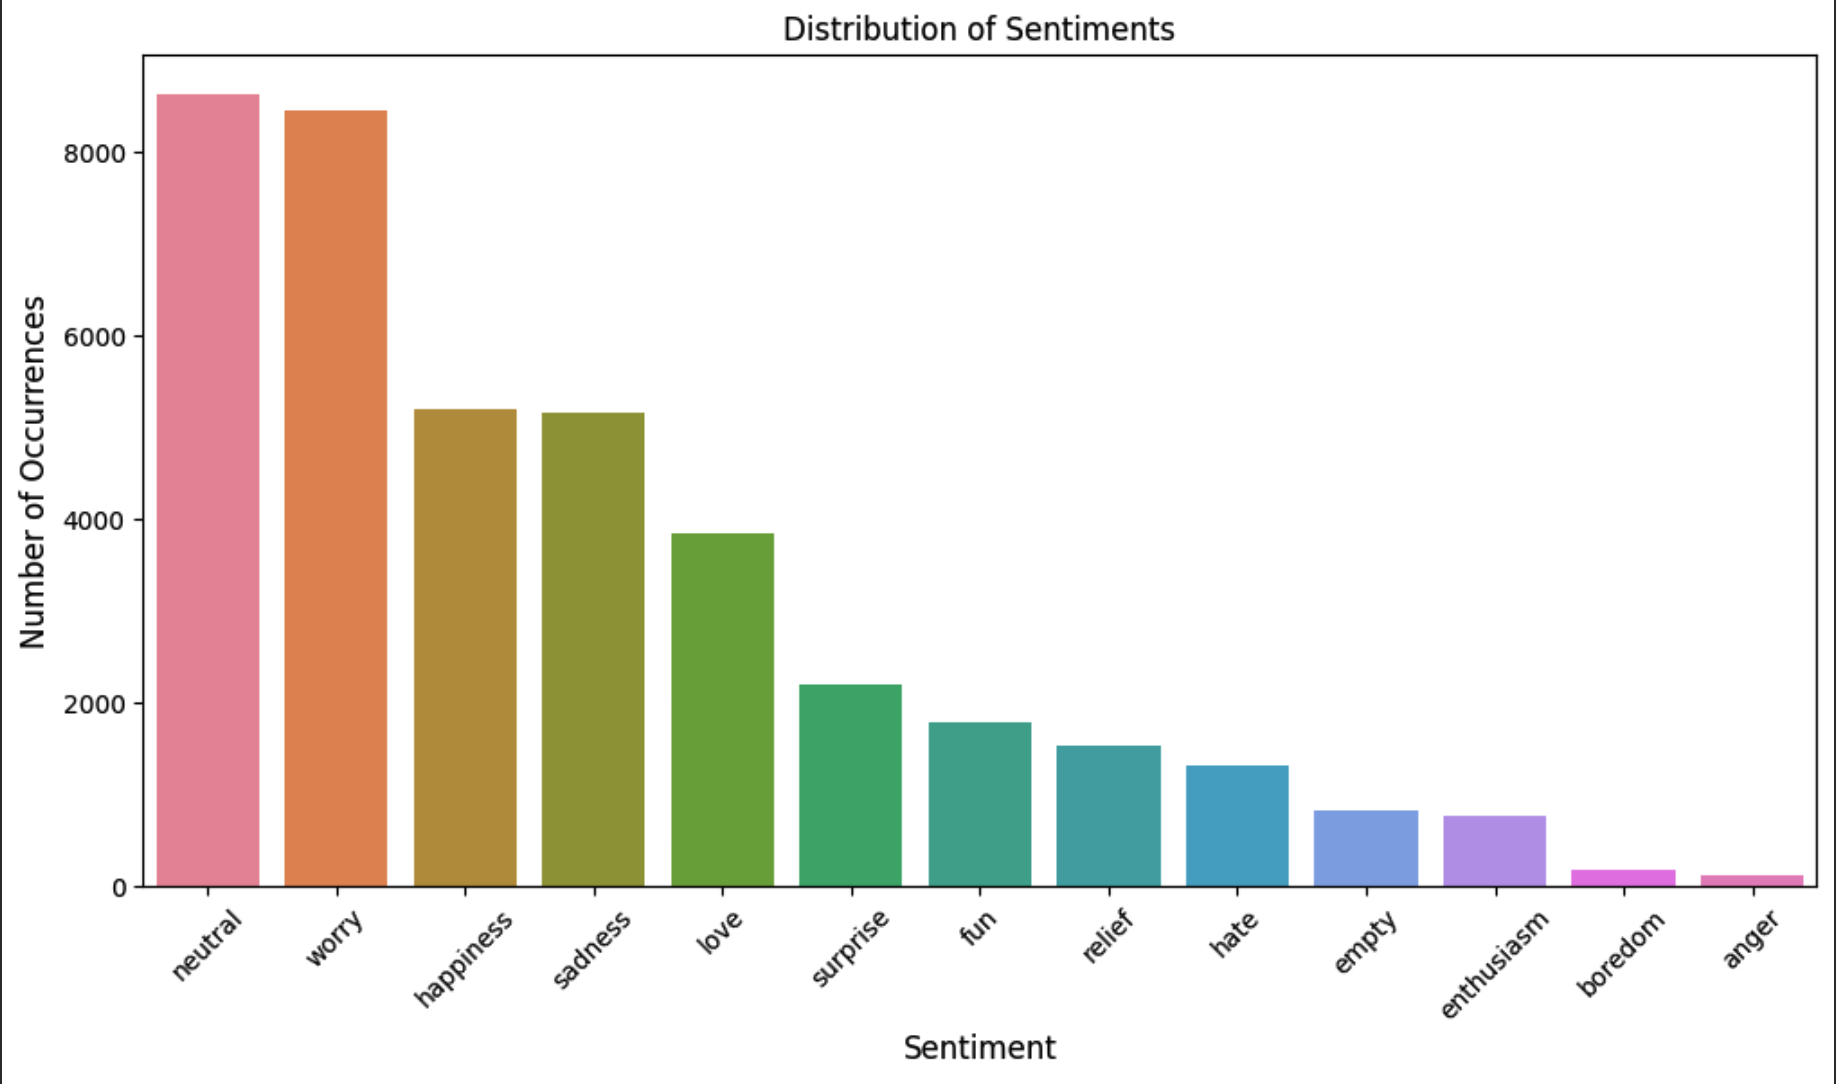
\includegraphics[width=0.8\textwidth]{path_to_sentiment_distribution.png}
\caption{Distribution of sentiments in the dataset}
\end{figure}

This visualization provides insights into the frequency of each sentiment in our dataset, indicating both the variety of sentiments and the volume of data available for each sentiment. This understanding is pivotal for the subsequent modeling phase.

\subsection{Modification}
Textual data requires thorough preprocessing. Our steps included:
\begin{itemize}
    \item Removal of special characters and numbers.
    \item Conversion to lowercase.
    \item Tokenization.
    \item Removal of stopwords.
    \item Lemmatization.
\end{itemize}
The sentiment labels were transformed into a numerical format using label encoding, as machine learning models require numerical input.

\subsection{Modeling}
Modeling is where prediction or classification algorithms are applied to the dataset. H2O's AutoML was employed due to its ability to automate the model selection and hyperparameter tuning processes. It evaluates a variety of models, selecting the top-performing ones based on a set criterion.\\

The top model, as per AutoML, was the Generalized Linear Model (GLM). GLM extends the ordinary linear regression model, allowing for various distributions of the error term, making it versatile for different types of data.\\

\begin{figure}[h]
\centering
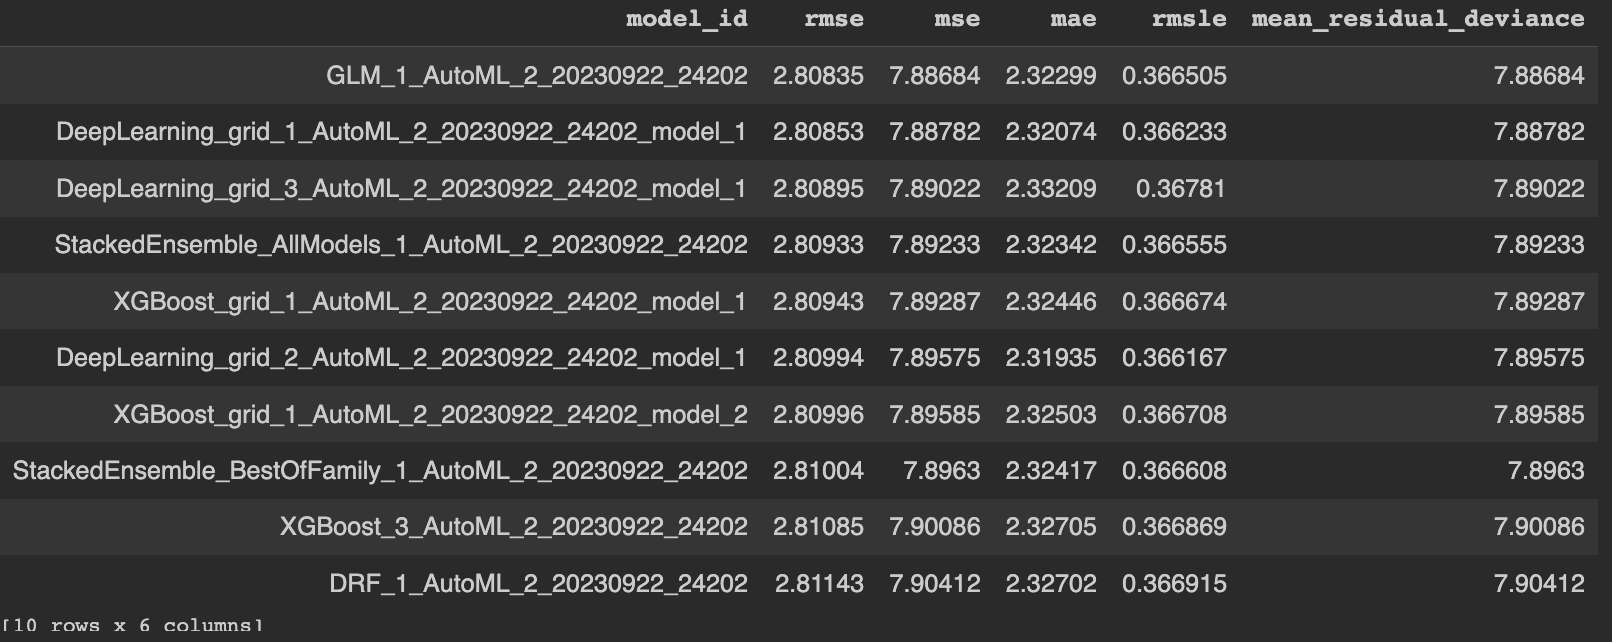
\includegraphics[width=0.8\textwidth]{path_to_glm_architecture.png}
\caption{Architecture of the Generalized Linear Model}
\end{figure}

\subsection{Assessment}
The models, once trained, underwent a rigorous assessment process. We used a withheld test dataset for this purpose, evaluating the models on various performance metrics. These metrics provide a detailed understanding of the model's capabilities. Specifically:
\begin{itemize}
    \item \textbf{MSE (Mean Squared Error):} Represents the average of the squares of the errors or deviations. It gives the error magnitude by penalizing large errors.
    \item \textbf{RMSE (Root Mean Squared Error):} Square root of MSE. It measures the average magnitude of the errors between predicted and observed values.
    \item \textbf{MAE (Mean Absolute Error):} Represents the average of the absolute differences between predicted and actual values. It provides a linear penalty for each unit of difference.
    \item \textbf{R-squared:} Indicates the proportion of the variance in the dependent variable that is predictable from the independent variables. It provides a measure of how well the model's predictions match the actual data.
\end{itemize}

\section{Results}
The GLM demonstrated commendable performance:
\begin{itemize}
    \item MSE: 8.0025
    \item RMSE: 2.8289
    \item MAE: 2.3415
    \item RMSLE: 0.3749
    \item R-squared: 0.0016
\end{itemize}

\begin{figure}[h]
\centering
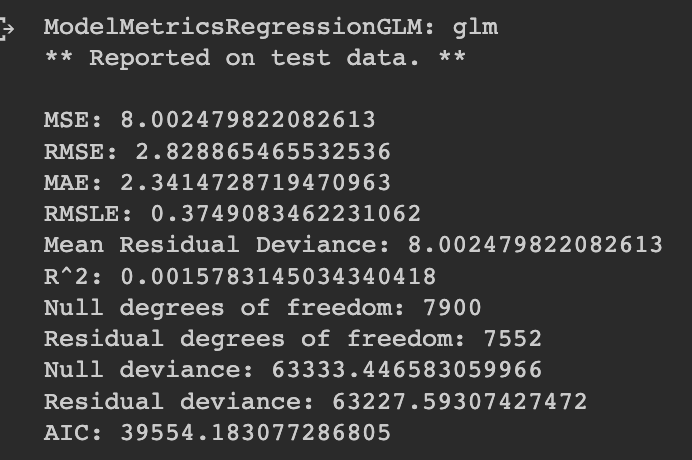
\includegraphics[width=0.8\textwidth]{path_to_result_visualization.png}
\caption{Visualization of the GLM's results}
\end{figure}

These results highlight the model's proficiency in emotion detection from textual data. The relatively low RMSE and MAE values suggest that the model's predictions are close to the actual values. The R-squared value, although low, is indicative of the variance explained by the model. Given the complexity of emotion detection and the nuances in textual data, these results are promising and indicate the potential applicability of the model in real-world scenarios.


\section{Conclusion}
By leveraging SEMMA and H2O's AutoML, we navigated the challenges of emotion detection from text. Our results underscore the significance of methodical data analysis and the power of machine learning in understanding human emotions.

\section{References}
\begin{enumerate}
    \item B. Pang and L. Lee. \textit{Opinion Mining and Sentiment Analysis}. Foundations and Trends in Information Retrieval, 2008.
    \item R. Feldman. \textit{Techniques and applications for sentiment analysis}. Communications of the ACM, 56(4):82–89, 2013.
    \item A. Go, R. Bhayani, and L. Huang. \textit{Twitter sentiment classification using distant supervision}. CS224N Project Report, Stanford, 2009.
    \item H2O.ai. \textit{H2O AutoML}. \url{https://docs.h2o.ai/h2o/latest-stable/h2o-docs/automl.html}, 2020.
    \item Kaggle. \textit{Emotion Detection from Text Dataset}. \url{https://www.kaggle.com/datasets/pashupatigupta/emotion-detection-from-text},
    \item K. Nigam, A. K. McCallum, S. Thrun, and T. Mitchell. \textit{Text classification from labeled and unlabeled documents using EM}. Machine learning, 39(2/3):103–134, 2000.
    \item I. Goodfellow, Y. Bengio, and A. Courville. \textit{Deep Learning}. MIT Press, 2016. \url{http://www.deeplearningbook.org}.
\end{enumerate}

\end{document}
